\section{System design}
\begin{figure}[t]
	\centering
	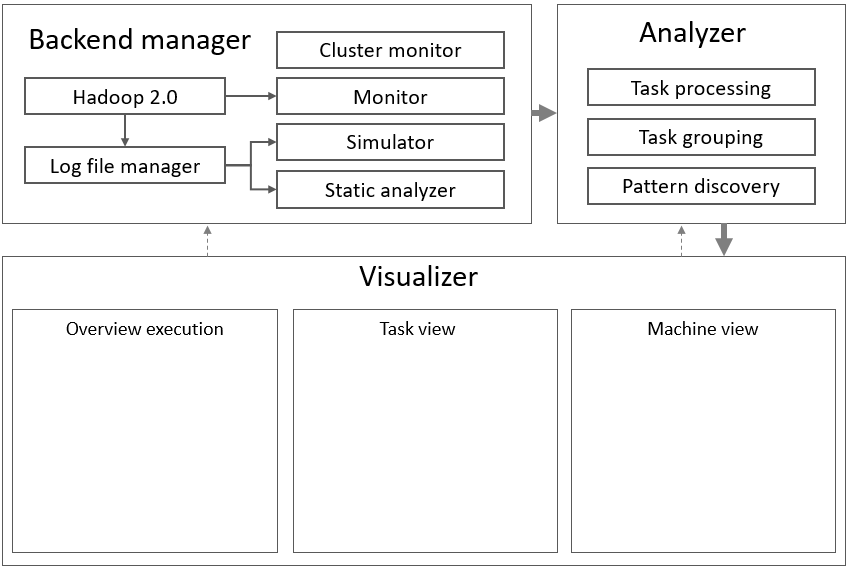
\includegraphics[width=0.45\textwidth]{figures/system/sysdesign.png}
	\vspace{-3mm}
	\caption{$\DQV$ system consists of three major components: backend manager, analyzer and visualizer.}
	\label{fig:sysdesign}
	\vspace{-3mm}
\end{figure}
As shown by Figure~\ref{fig:sysdesign}, $\DQV$ consists of three modules: backend manager, analyzer, and visualizer. 

In our current system, we use Hadoop2.0 as the\textbf{ distributed query engine}. The system can run in three mode: monitoring mode, simulation mode and analytics mode. The monitoring mode directly collect the real-time execution log from Hadoop2.0, then process it and send the result to analyzer. The simulator and log analyzer are linked with log file manager, a module to process and save logs as as structured data form at local disk. The simulator will simulate the execution progress which allow users to explore the dynamic process.

\subsection{System overview}
